% Search for XXXX for places which you need to add your contributions. 

\documentclass{article}
\usepackage{graphicx}
\title{COMP20010 Lab Six: Algorithm Analysis}
\author{Kashif Hussain}
\begin{document}
\maketitle

%to make the graphs show use the following method:
%latex analysis.tex -> analysis.dvi
%dvips analysis.dvi -> analysis.ps
%ps2pdf analysis.ps -> analysis.pdf

% LAB 6 PART 1
\section{Part~1 Algorithm}
\label{sec:algorithm1}

\subsection{Asymptotic run-time analysis}

My algorithm runs in asymptotic time $O(nLogn)$. The argument for this follows:

The storing of values requires n comparisons of i to n. (i < n for loop)
i++ is executed n-1 times (increments and stores -> 2n-2 (for loop)
scanf executes n times
indexing an array occurs n times
storing a value occurs n times.

This means the for loop is $O(n + 2(n-1) + n + n + n)$ = $O(6n-2)$ = $O(cn)$ = $O(n)$

The quicksort algorithm has best/average case of O(nlogn) but the worst case is
$O(n^2)$.
This is because:
The partition operation takes O(n).
In the most unbalanced case, each time we perform a partition we divide the 
list into two sublists of size 0 and n-1 
(for example, if all elements of the array are equal). 
This means each recursive call processes a list of size one less than the 
previous list. Consequently, we can make n-1 nested calls before we reach a 
list of size 1. This means that the call tree is a linear chain of n-1 nested
calls. The ith call does O(n-i) work to do the partition, and
sum from i=0 to n of (n-i) = $O(n^2)$, so in that case Quicksort takes 
$O(n^2)$ time. That is the worst case

So the quicksort takes $O(n^2)$ (Worst Case)

While loop:
Worst case involves it searching from the 90th percentile value to the last
value in the array (if the numbers in the range of the 90th percentile to the 
final are the same value including the final number) to produce a -1.

This means while (found == 0) is checked 0.1*n times 
(0.1* = final 10\% of values)
the (numbers[nextInteger] > numbers[ninetyPercentileArrayNo]) comparison takes
place 0.1*n times
nextInteger = nextInteger +1 is 2 operations (summing and storing) and so occurs
2*0.1*n times

Worst case is: $O((0.1*n) + (0.1*n) + (2*0.1*n))$ = $O(0.4n)$ = $O(n)$ = $O(n)$

This gives a final asymptotic time of:

$O(n^2 + n + n)$ = $O(n^2 +2n)$ =  $O(n^2)$ (Worst Case)
$O(nlogn + n + n)$ = $O(n(logn + 2))$ = $O(nlogn)$ (Average Case)

\newpage
\subsection{Experiments}
\label{sec:experiments1}

I will be using real time for my experiments.

% If you put your results in a graph, uncomment the following. 

 \begin{figure}
   \centering
 \resizebox{0.9\textwidth}{!}{\includegraphics{my-plot1.ps}}  
  
   \caption{Error plot of different inputs for Algorithm 1}
   \label{fig:experiment1}
 \end{figure}

\begin{figure}
   \centering
 \resizebox{0.9\textwidth}{!}{\includegraphics{my-plot1.ps}}  
  
   \caption{Fitplot of different inputs for Algorithm 1}
   \label{fig:experiment2}
 \end{figure}

As you can see, as n gets larger, the shape of the graph approximates to nlogn
The gradient from x = 100000 to 3000000 is 1
This  tells me that the power of n is 1.
Using fitscript i get: a = 1.96323e-08 for f(N) = 1.96323e-08 * N * log(N)

% If you put your results in a table, the followin might be helpful. 
% Replace the formula in the third column with the formula you are testing. 

 \begin{center}
 \begin{tabular}{l||l|l|}
   data size   & run time    & $t = 1.96323e-08*N*log(N)$       \\  \hline
   100000      &0.031            0.0293                \\
   500000			 &0.14583					 0.1466						     \\
   1000000		 &0.28967					 0.2933						     \\
   1500000		 &0.43586				   0.4400							   \\
   2000000	   &0.57573					 0.5866							   \\
   2500000		 &0.72089					 0.7333						     \\
   3000000     &0.8597           0.8800                \\

\end{tabular}
 \end{center}

the difference in run time in steps of 500000 gradually decreases
500000 to 1000000 -> Approx 0.145 increase
1500000 to 2000000 -> Approx 0.140 increase
2500000 to 3000000 -> Approx 0.135 increase

The graph of nlogn tends to curve down for high values of n and shows a pattern
of doing so. Every step of 500000 has a smaller and smaller increase in runtime
\subsection{Prediction}
\label{sec:prediction1}
%t(N) = 0.00000088*1000000^1/3 better approx
My estimate of the equation for the run-time of the algorithm is:
\begin{equation}
  \label{eq:estimated_runtime1}
   t(N) = 1.96323e-08*N*log(N)
\end{equation}

Using this, the estimated time to find the ninetieth percentile of a
file containing 60 million numbers is 30.44 seconds.


%LAB 6 PART 2
\section{Part~2 Algorithm}
\label{sec:algorithm2}

\subsection{Asymptotic run-time analysis}

My algorithm runs in asymptotic time $O(N)$. 

The argument for this follows:

The for loop which scans a file for integers does the following:
The storing of values requires n comparisons of i to n. (i < n for loop)
i++ is executed n-1 times (increments and stores) (for loop)
scanf executes n times
storing a value in variable value occurs n times
checking if value is greater than or equal to 1000000 occurs n times
storing the values and indexing an array occurs k times (where k = n-x)
This means the for loop is $O(n + 2(n-1) + n + n + n + k)$ = $O(6n-2 + k)$ = $O(cn)$ = $O(n)$

The least significant radix sort has a worst case perfomance of O(kN)

Indexing and storing variables in the 2nd array does the following:
k = the number of values >= 1000000 in N. (k=n-x)

makes k comparisons (i<k)
makes k-1 incrmements and storage operations (i++)
index's and stores a value k times (number2[i] = numbers[i])

$O(n-x + 2(n-x-1) + 2(n-x))$ = $O(5n-4x-2)$ = $O(cn)$ = $O(n)$

In total this gives:

$O(n + kn + n)$ = $O(n)$

\subsection{Experiments}
\label{sec:experiments2}

I will be using real time for my experiments
% If you put your results in a graph, uncomment the following. 

 \begin{figure}
   \centering
 \resizebox{0.9\textwidth}{!}{\includegraphics{my-plot2.ps}}  
  
   \caption{Error plot of different inputs for Algorithm 2}
   \label{fig:experiment3}
\end{figure}

\begin{figure}
   \centering
 \resizebox{0.9\textwidth}{!}{\includegraphics{my-fit2.ps}}  
  
   \caption{Fit plot of different inputs for Algorithm 2}
   \label{fig:experiment4}
\end{figure}

As you can see, as n gets larger, the shape of the graph approximates to n
The gradient from x = 1 to 1000000 is 1
This tells me that the power of n is 1.
Using fitscript i get: a = 1.2563e-07 for f(N) = 1.2563e-07 * N 

% If you put your results in a table, the followin might be helpful. 
% Replace the formula in the third column with the formula you are testing. 

 \begin{center}
 \begin{tabular}{l||l|l|}
   data size   & run time    & $t = 1.2563e-07*N$       \\  \hline
   100000      &0.0150           0.0126                \\
   500000			 &0.0730				   0.0628						     \\
   1000000		 &0.1278					 0.1256						     \\
   1500000		 &0.1958				   0.1884							   \\
   2000000	   &0.2522					 0.2513							   \\
   2500000		 &0.3107					 0.3141						     \\
   3000000     &0.3729           0.3767                \\

\end{tabular}
 \end{center}

the difference in run time in steps of 500000 remains approximately constant

500000 to 1000000 -> Approx 0.0628 increase
1500000 to 2000000 -> Approx 0.0629 increase
2500000 to 3000000 -> Approx 0.0626 increase

As the increase in steps of 500000 remains constant, it follows the pattern
of f(N) = aN where a remains constant.


\subsection{Prediction}
\label{sec:prediction2}

My estimate of the equation for the run-time of the algorithm is:
\begin{equation}
  \label{eq:estimated_runtime2}
  $t(N) = 1.2563e-07*N$
\end{equation}
Using this, the estimated time to find the ninetieth percentile of a
file containing 60 million numbers is 7.54 seconds.

\end{document}
